\section[Le architetture]{Le architetture}
\sectionframe{images/covers/cover_architecture.jpeg}{Le Architetture}
% Seattle Public Library Central Library, Seattle, United States: https://unsplash.com/it/foto/if2coegqwZU by Chance Anderson

\subsection[L'architettura di un computer]{L'architettura di un computer}


\begin{frame}
	\frametitle{L'architettura di un computer}
	 
	\begin{block}{Il computer}
		Il computer è un dispositivo fisico che implementa il funzionamento di una macchina di Turing.
	\end{block}
	\begin{block}{La Macchina di Turing}
		La Macchina di Turing è una macchina ideale che manipola i dati contenuti su un nastro di lunghezza potenzialmente infinita, secondo un insieme prefissato di regole ben definite.\\
		In altre parole, si tratta di un modello astratto che definisce una macchina in grado di eseguire algoritmi e dotata di un nastro potenzialmente infinito su cui può leggere e/o scrivere dei simboli.
	\end{block}
\end{frame}


\begin{frame}
	\frametitle{La macchina di Turing}
	
	\begin{block}{Una simulazione della Macchina di Turing}
		\begin{figure}[!htbp]
			\centering 
			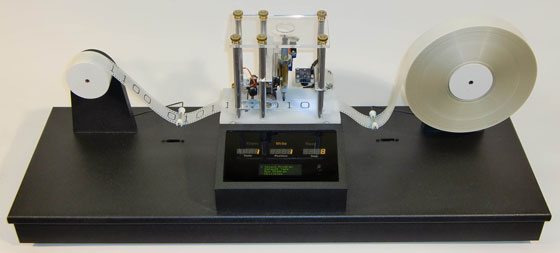
\includegraphics[width=0.9\linewidth]{images/2_le_architetture/turing_machine.jpg}
			\caption{Foto da \href{https://aturingmachine.com/}{aturingmachine.com}, clicca \underline{\href{https://www.youtube.com/watch?v=E3keLeMwfHY}{qui}} per vedere il video.}
		\end{figure}
	\end{block}
\end{frame}


\begin{frame}
	\frametitle{Il computer}
	
	\begin{block}{Il computer}
		Un computer esegue programmi (come la macchina di Turing).\\
		Esistono due categorie di computer:
		\begin{columns}			
			\column{0.3\linewidth}
			\begin{figure}[!htbp]
				\centering 
				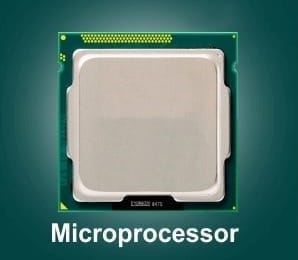
\includegraphics[width=0.7\linewidth]{images/2_le_architetture/microprocessor.jpeg}
				%\caption{}
			\end{figure}
			
			\column{0.5\linewidth}
			$\bullet$ \textbf{general purpose}:\\riprogrammabili dall'utente ($\mu$processors).
			
			\column{0.2\linewidth}
			\begin{figure}[!htbp]
				\centering
				\advance\leftskip-0.5cm
				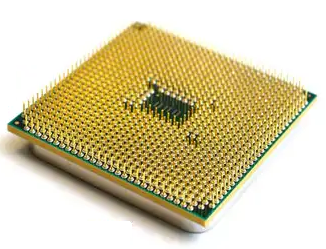
\includegraphics[width=1.0\linewidth]{images/2_le_architetture/microprocessor.png}
				%\caption{}
			\end{figure}
			
		\end{columns}
		 
		\begin{columns}						
			\column{0.3\linewidth}
			\begin{figure}[!htbp]
				\centering 
				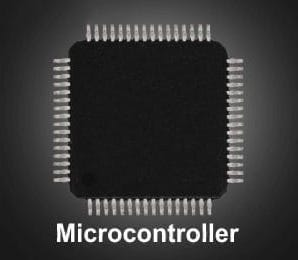
\includegraphics[width=0.7\linewidth]{images/2_le_architetture/microcontroller.jpeg}
				%\caption{}
			\end{figure}
			
			\column{0.5\linewidth}
			$\bullet$ \textbf{special purpose}:\\dedicati ad una sola applicazione specifica  ($\mu$controllers).
			
			\column{0.2\linewidth}
			\begin{figure}[!htbp]
				\centering
				\advance\leftskip-0.5cm
				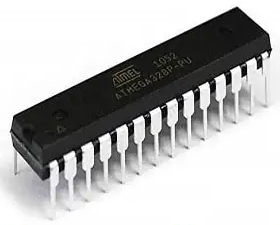
\includegraphics[width=1.0\linewidth]{images/2_le_architetture/microcontroller.png}
				%\caption{}
			\end{figure}
			
		\end{columns}
		
	\end{block}
	
	
\end{frame}



\subsection[I Transistor]{I Transistor}
\begin{frame}
	\frametitle{I Transistor}
	
	\begin{columns}			
		\column{0.6\linewidth}
		\begin{block}{I microprocessori e i microcontrollori}
			I microprocessori e i microcontrollori sono componenti chiave dei computer e dei dispositivi elettronici in quanto ne costituiscono il "cervello".\\
			Uno dei componenti elettronici più importanti all'interno di questi sono i \textbf{transistor}.
		\end{block}
		
		\column{0.4\linewidth}
		\begin{figure}[!htbp]
			\centering 
			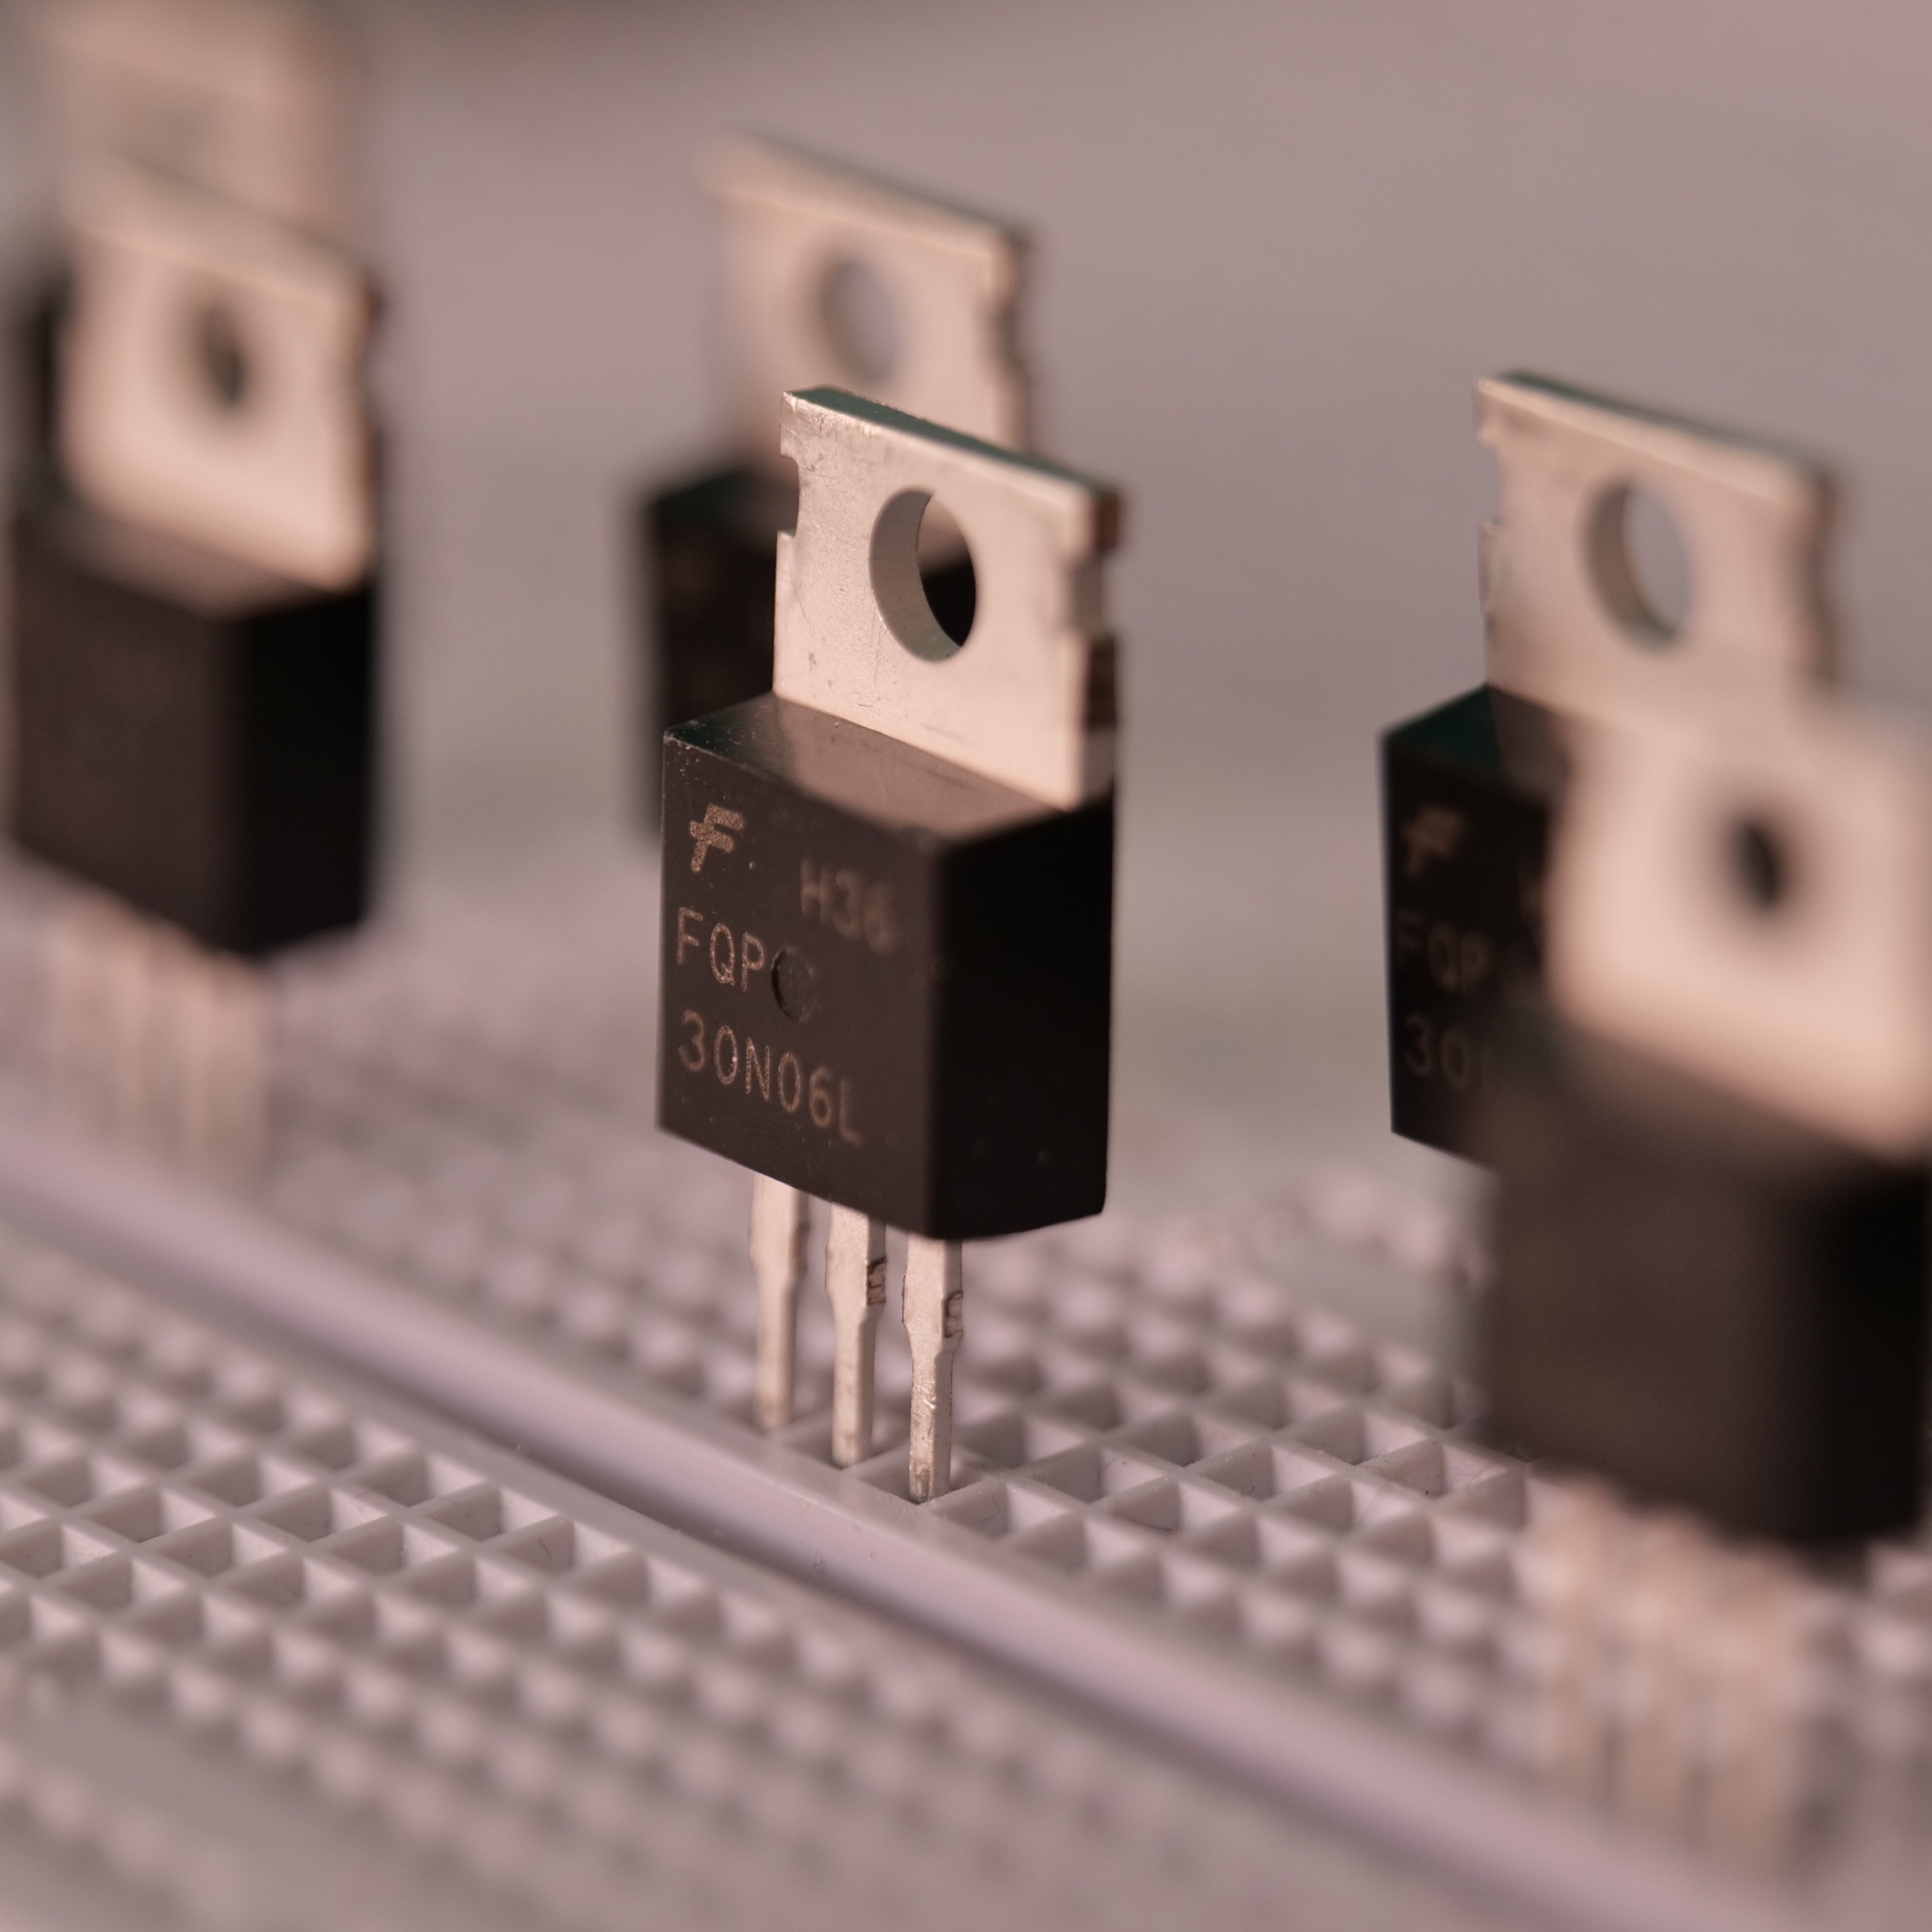
\includegraphics[width=0.95\linewidth]{images/2_le_architetture/transistor.jpg}
			\caption{Foto di \href{https://unsplash.com/it/@trisolarian}{Axel R.}}
		\end{figure}		
	\end{columns}
	
\end{frame}




\begin{frame}
	\frametitle{I Transistor}
	
	\begin{columns}			
		\column{0.6\linewidth}
		\begin{block}{I Transistor}
			I transistor sono componenti elettronici utilizzati in molti circuiti elettronici in quanto permettono di \textbf{amplificare} o \textbf{interrompere} un \textbf{segnale elettrico}.
		\end{block}
		
		\begin{block}{16 Dic 1947, Bardeen, Brattain e Shockley riuscirono a creare il primo transistor}
			all'interno degli \textbf{AT\&T Bell Laboratories} (un centro di ricerca e sviluppo, attualmente di proprietà di Nokia) da allora sono diventati un componente chiave dell'elettronica.
		\end{block}
		
		\column{0.4\linewidth}
		\begin{figure}[!htbp]
			\centering 
			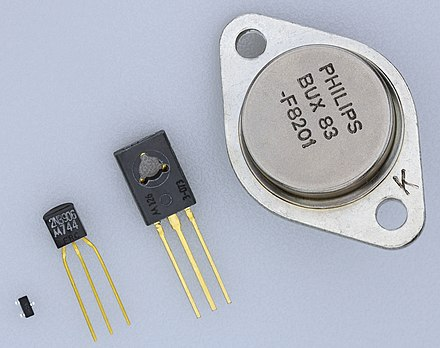
\includegraphics[width=0.95\linewidth]{images/2_le_architetture/transistors.jpg}
			\caption{Confronto tra diversi transistor BJT, da sinistra a destra: SOT-23, TO-92, TO-126, TO-3}
		\end{figure}		
	\end{columns}
	
\end{frame}



\begin{frame}
	\frametitle{I Transistor}
	
	\begin{columns}			
		\column{0.6\linewidth}
		\begin{block}{Il Nobel}
			Il transistor doveva inizialmente servire a \textbf{migliorare le comunicazioni} tra il continente americano e quello europeo oggi lo troviamo impiegato nei campi più disparati (informatica, telefonia, smart-car, radio, ...).\\~\\
			Nel \textbf{1956} i tre scienziati statunitensi hanno ricevuto il \textbf{Premio Nobel per la Fisica} per gli studi condotti all'interno dei laboratori di ricerca e sviluppo dell'AT\&T: in appena 9 anni il transistor è diventato una delle componenti hardware più importanti e utilizzate in ambito elettronico.
		\end{block}
		
		\column{0.4\linewidth}
		\begin{figure}[!htbp]
			\centering 
			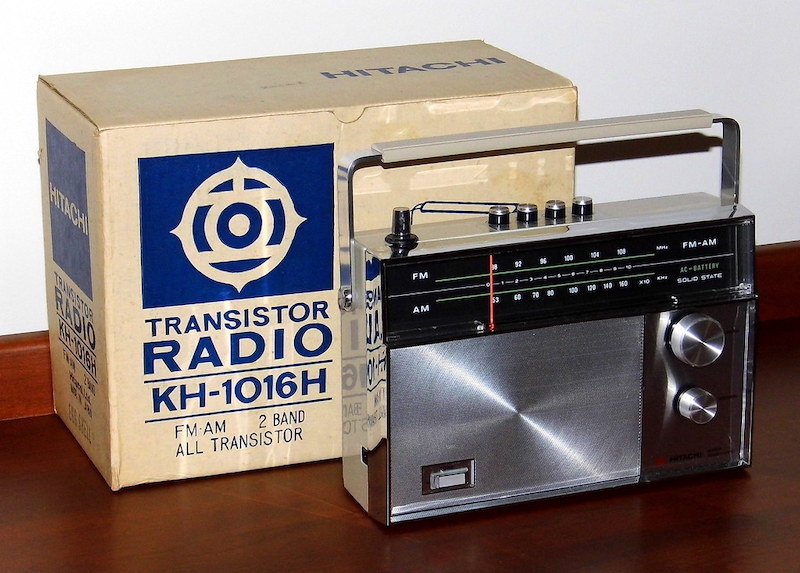
\includegraphics[width=0.95\linewidth]{images/2_le_architetture/radio_transistors.jpeg}
			\caption{I transistor sono usati nelle radio sia per amplificare il segnale radiofonico   ricevuto dall'antenna che per il circuito di sintonizzazione utilizzato per selezionare la frequenza del segnale radiofonico.}
		\end{figure}		
	\end{columns}
	
\end{frame}


\subsection[La capacità di integrazione]{La capacità di integrazione}
\begin{frame}
	\frametitle{La capacità di integrazione}
	
	\begin{block}{La capacità di integrazione}
	
	\end{block}
	
\end{frame}


\subsection[La legge di Moore]{La legge di Moore}
\begin{frame}
	\frametitle{La legge di Moore}
	
	\begin{block}{La legge di Moore}
	
	\end{block}
	
\end{frame}
